\documentclass[conference]{IEEEtran}

\usepackage{amsmath,amssymb,amsfonts}
\usepackage{graphicx}
\usepackage{textcomp}
\usepackage{xcolor}

\usepackage[inline]{enumitem}
\usepackage[]{algorithm2e}
\usepackage[doi=false, isbn=false, url=false, natbib=true, style=ieee, backend=bibtex]{biblatex}
\usepackage{float}
\usepackage[draft]{hyperref}
\hypersetup{
    % draft,
    colorlinks,
    linkcolor={black!50!black},
    citecolor={blue!50!black},
    urlcolor={blue!80!black}
}
\usepackage[acronym, toc, nonumberlist]{glossaries}

\renewcommand{\figurename}{Figure}

% Hyperlink figures and algorithms
\newcommand{\figref}[1]{\hyperref[#1]{\figurename~\ref*{#1}}}
\newcommand{\algref}[1]{\hyperref[#1]{Algorithm~\ref*{#1}}}

% define image width
\newcommand{\imageWidth}{0.45} 

\addbibresource{references.bib}

\makeglossaries
\newacronym{iot}{IoT}{Internet of Things}
\newacronym{coap}{CoAP}{The Constrained Application Protocol}
\newacronym{udp}{UDP}{User Datagram Protocol}
\newacronym{rest}{REST}{Representational State Transfer}
\newacronym{m2m}{M2M}{Machine-to-Machine}
\newacronym{rpi}{RPi}{Raspberry Pi}
\newacronym{json}{JSON}{JavaScript Object Notation}
\newacronym{gpio}{GPIO}{General Purpose Input Output}
\newacronym{dtls}{DTLS}{Datagram Transport Layer Security}
\newacronym{uri}{URI}{Uniform Resource Identifier}
\newacronym{http}{HTTP}{HyperText Transfer Protocol}
\newacronym{api}{API}{Application programming interface}
\newacronym{mqtt}{MQTT}{Message Queuing Telemetry Transport}
\newacronym{wsn}{WSN}{Wireless Sensor Network}
\newacronym{aws}{AWS}{Amazon Web Services}
\newacronym{ssl}{SSL}{Secure Socket Layer}

\def\BibTeX{{\rm B\kern-.05em{\sc i\kern-.025em b}\kern-.08em
    T\kern-.1667em\lower.7ex\hbox{E}\kern-.125emX}}
\begin{document}

\title{CoAP based IoT data transfer from a Raspberry Pi to Cloud}

\author{\IEEEauthorblockN{Thomas Lee Scott}
\IEEEauthorblockA{\textit{School of Computing, Mathematics \& Digital Technology} \\
\textit{Manchester Metropolitan University}\\
Manchester, United Kingdom \\
tomscott292@gmail.com}
\and
\IEEEauthorblockN{Amna Eleyan}
\IEEEauthorblockA{\textit{School of Computing, Mathematics \& Digital Technology} \\
\textit{Manchester Metropolitan University}\\
Manchester, United Kingdom \\
A.Eleyan@mmu.ac.uk}
}

\maketitle

\begin{abstract}
This research investigates the use of \gls{coap} in transmitting sensor data
to the cloud. It aims to explore how \gls{coap} fits into the \gls{iot} ecosystem and
what advantages, if any, it offers over other \gls{iot} protocols. A framework is proposed 
using a \gls{rpi} and sensor acting as an \gls{iot} endpoint. This endpoint will allow for
\gls{coap} requests and will poll the sensor and return the latest data as \gls{json}.
The endpoint will be polled from a cloud service, this service will then display the data to 
the user.
\end{abstract}

\begin{IEEEkeywords}
Internet of Things, CoAP, M2M, constrained devices, Raspberry Pi board.
\end{IEEEkeywords}

\section{Introduction}
The reduced cost of low powered small devices, such as the \gls{rpi}, has made it more accessible to create bespoke systems. 
This combined with the increasing popularity of home automation allows for these devices to be used in the \gls{iot}.

The \gls{iot} can be viewed as a large distributed network comprising of highly dynamic devices \citep{miorandi2012internet}. Small low powered ``smart'' devices can connect and communicate with one another. Some of these devices can contain or communicate with sensors that record real world data. This data can then be transmitted to other devices allowing them to trigger actions. In this way groups of smart devices can be used to improve day to day situations such as automated houses (thermostats and heating etc.), security and improved monitoring.

The Raspberry Pi \citep{pi3model} is a credit card sized computer developed by the Raspberry Pi Foundation. 
The \gls{rpi}'s ability to act as a GNU/Linux server and the interfacing services provided by its general purpose I/O pins make it a popular 
choice of hardware for \gls{iot} applications. \citep{kumar2016iot}

With 48\% of the UK market considering their smartphone as the most important device for internet access \citep{ofcom2018} allowing users to use their handheld devices to view and manage their data has become increasingly necessary. Cloud platforms that allow access from any device go a long way to 
solving this problem. Storing sensor data in the cloud allows for easy access to users from any device as well as allowing for scalable storage.

As these devices are limited in computing power it is important that the devices communicate efficiently. 
This paper explores the use of \gls{coap} as a protocol to transmit sensor data from a small, low powered device (\gls{rpi}) to send sensor data to the cloud.

In this system the a sensor will be attached to the \gls{rpi}, the \gls{rpi} will be responsible for taking the data from the sensor and then 
using the \gls{coap} protocol to transmit this data to the cloud platform.

\subsection{Motivation}
With the increasing adoption of \gls{iot} systems and technology in day to day
life, it becomes increasingly important for the devices to be able to operate
at peak efficiency. As there are numerous technologies and standards that allow
different \gls{iot} devices to communicate, this paper investigates the use
of \gls{coap} in order to determine:
\begin{enumerate*}
    \item how \gls{coap} transfers data from a \gls{iot} device to another \gls{coap} node.
    \item how a \gls{rpi} can be used as a flexible platform to provide sensor data.
    \item how this data can be sent to a cloud platform.
\end{enumerate*}

\subsection{Related Work and Contribution}
\cite{rode_iot_2017} carries out a similar investigation, using a \gls{rpi} 
device as a \gls{iot} node connected to sensors. The \gls{rpi} collects the 
data from the sensors and then transmits the data to a cloud platform. The 
cloud platform in this instance is a \gls{http} server which will receive the
sensor data and display it to the user. \cite{rode_iot_2017} proposes using the 
\gls{mqtt} protocol to transmit the sensor data from the \gls{rpi} to the
\gls{http} server.
\gls{mqtt} is a popular \gls{iot} protocol developed to specialise in the transfer
of data from \glspl{wsn} \citep{hunkeler_mqtt-s_2008}. \gls{mqtt} works on a 
publish/subscribe model, in \cite{rode_iot_2017} the \gls{rpi} acts a \textit{publisher}, 
publishing the sensor data to the broker and the \gls{http} server acts as a
\textit{subscriber}. The \gls{mqtt} broker is responsible for coordinating subscribers 
to the data and subscribers will usually have to contact the broker explicitly in 
order to subscribe \citep{hunkeler_mqtt-s_2008}.
This contrasts to the approach taken in this proposal using \gls{coap}, Where each
node in the \gls{coap} network acts as both a server and a client in a more traditional
\gls{http} model and nodes within the infrastructure will communicate with one
another directly.

\cite{jassas_smart_2015} used a \gls{rpi} connected to sensors to measure 
patient's body temperature and transmit this data wirelessly to the cloud.
In that paper, the data was transmitted to a \gls{aws} cloud computing platform
where the data was stored, mined in order to make decisions based on the data 
and provided a service for updating, reviewing and displaying the data to users.
The data was transmitted from the \gls{rpi} to the \gls{aws} server using \gls{ssl}.
The development of specialised protocols for constrained devices, such as \gls{coap}
and \gls{mqtt} could allow these health monitoring \glspl{rpi} to save power,
save network bandwidth and potentially receive more readings to process.

\cite{lee_internet_2018} used a \gls{rpi} combined with a DHT22 sensor to measure
the indoor temperature in real time. This data was transmitted using \gls{http}
to a \gls{rest} \gls{api} where the temperature was stored in a database.
These temperatures were then used to inform an application replicating 
the actions of an air conditioner. The use of a \gls{rest}ful \gls{api} in 
this paper would allow the project to easily be adapted to using \gls{coap} 
to replace \gls{http}.

Most of the above related \gls{iot} architectures are deployed 
using either \gls{mqtt} or \gls{http}.
However, this paper proposes a \gls{coap}--based \gls{iot} architecture, 
which uses \gls{coap} to transmit sensor data from \gls{rpi} 
to ThingsBoard \gls{iot} cloud platform to monitor and 
visualise sensor devices and share it with users.

\section{Background}
\subsection{Internet of Things}
The \acrfull{iot} is an umbrella term used to describe physical `smart' devices
equipped with telecommunication interfaces, connected to one another via the 
Internet \citep{centenaro_long-range_2016}.
Whereas the Internet traditionally connected computers, the embedding of 
electronics into physical objects has allowed the Internet to expand \citep{miorandi_internet_2012}.
These devices can contain sensors which will produce data and in some cases, 
these devices can be controlled remotely. The combination of these devices in
a network, especially when the actions of one device are informed by the 
data from another device, is the foundation of \gls{iot} \citep{minerva_towards_2015}.
\gls{iot} systems can impact in many areas such as home automation,
where devices can work together to automate heating and security aspects of 
the home \citep{lee_internet_2018}, and medicine where devices
can be used as monitors to provide real-time information about 
patient health \citep{kumar_iot_2016}.

\begin{figure}[H]
    \centering
    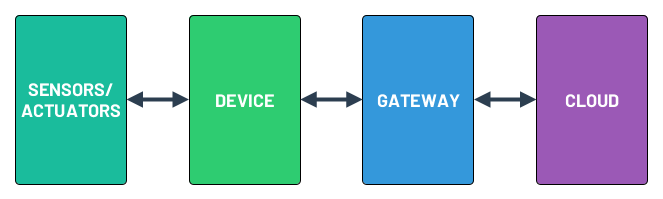
\includegraphics[width=\imageWidth\textwidth]{assets/generic_iot_architecture.png}
    \caption{\label{fig:generic_iot_architecture} Basic \gls{iot} Architecture.}
\end{figure}

Although \gls{iot} lacks a standardized architecture approved by an authorized
body \citep{minerva_towards_2015},
\figref{fig:generic_iot_architecture} illustrates various common
components present within any given \gls{iot} architecture.
The sensor/actuator is the component that will receive data from the real 
world or perform a physical action. 
This data is then transmitted to a device which is
responsible for the sensor/actuator.
The device may be responsible for multiple sensors,
as in \citet{jassas_smart_2015},
which connected multiple e-health sensors to a single \gls{rpi} device.
This device will then communicate with a gateway.
The gateway is responsible for ensuring that 
the data is sent to the correct destination. 
Within \gls{coap}, the gateway would be a router ensuring messages are sent 
to the correct endpoints. The cloud is the final destination for the sensor data; 
here, the data will be stored and can be processed for further analysis.


\subsection{The Constrained Application Protocol}
\acrfull{coap} is a transfer protocol specialised for use with the web, constrained
nodes and constrained networks \citep{shelby_constrained_2014}. The protocol is 
designed for \gls{m2m} applications and is ideally suited for use within the 
\gls{iot} ecosystem. \glspl{coap} features of observable resources, multicasting, \gls{m2m} discovery 
make it a better fit for \gls{iot} applications than \gls{http} \citep{kovatsch_californium:_2014}.

\gls{coap} recognises that web services have become dependant in \gls{rest} 
architecture and works to implement a subset of \gls{rest} common with HTTP while
optimising for \gls{m2m} applications \citep{shelby_constrained_2014}. It achieves 
this by offering built-in discovery, multicast support and asynchronous message 
exchanges \citep{shelby_constrained_2014}. 

\gls{coap} uses a compact binary format with a fixed header size of 4 bytes, 
exchanging messages over \gls{udp} or \gls{dtls} to send messages securely. \gls{coap} 
resources are addressable by \glspl{uri} and can be interacted with through the 
same methods as \gls{http}: GET, PUT, POST and DELETE.

With regards to reliability, \gls{coap} offers four types of messages: Confirmable, 
Non-Confirmable, Acknowledgement and Reset \citep{bellavista_towards_2016}.
After a Confirmable request is sent to a \gls{coap} endpoint, the endpoint will 
respond with an Acknowledgement message. This message can contain the requested 
data in a `piggybacked' response. Otherwise, an empty Acknowledgement message is sent 
and a Confirmable message will be sent once the data is ready. The original
requester will then respond with an empty Acknowledgement message to confirm receipt 
of the data \citep{shelby_constrained_2014}.


\section{Designed \gls{coap}-based \gls{iot} Architecture}
The system shall consist of four main elements: the sensor, the \gls{rpi}, \gls{coap} and the cloud platform.
The sensor will collect the data and pass this to the \gls{rpi}. The \gls{rpi} will then be responsible for manipulating
the data into a suitable format for transmission via \gls{coap}. The implementation of \gls{coap} will communicate with
the cloud platform. The cloud platform will store the data, allowing access to users.

\begin{figure}[H]
    \centering
    \makebox[1\textwidth]{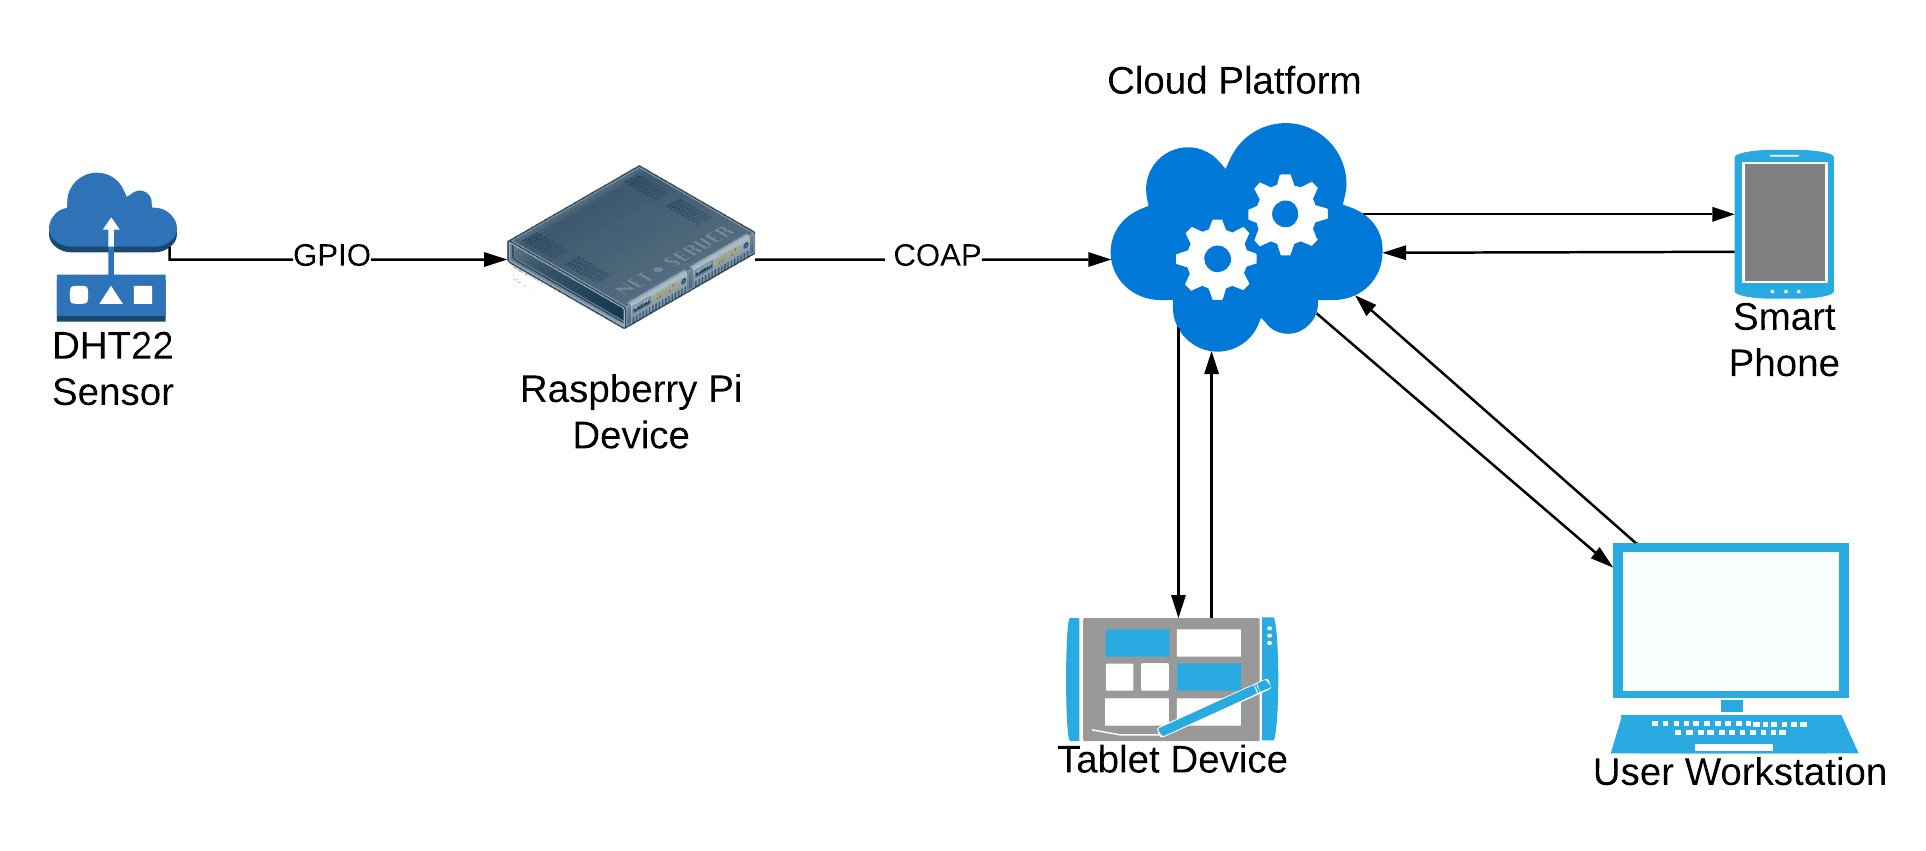
\includegraphics[width=1\textwidth]{assets/Project_Framework.png}}
    \caption{\label{fig:proj_framework} The project infrastructure.}
\end{figure}

The DHT22 sensor will connect to the \gls{rpi} using the \gls{rpi}'s on board \gls{gpio} ports as shown in \figref{fig:rpi_wiring}. 
A Python script using the AdaFruit Python DHT package to retrieve data from the sensor and the CoAPthon Python library will format the sensor data as 
\gls{json}. This script will then make the \gls{json} data available as a \gls{coap} endpoint from which the cloud service can get or subscribe to 
the latest data. 


\begin{figure}[H]
    \centering
    \makebox[1\textwidth]{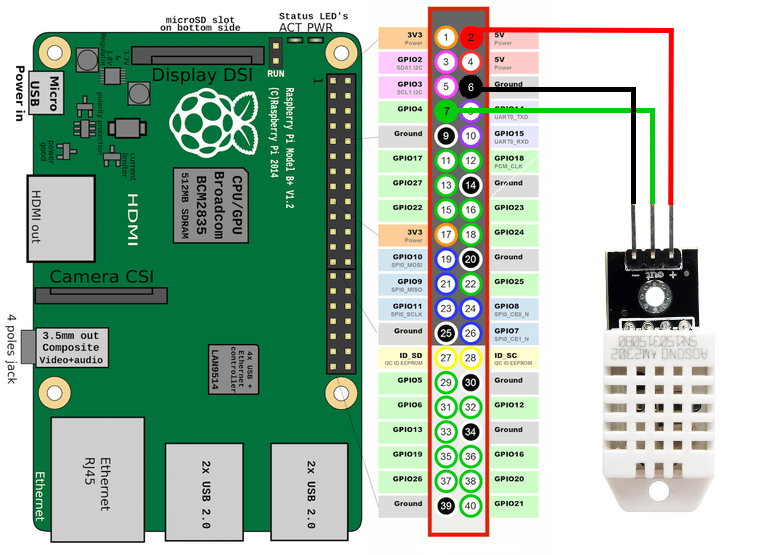
\includegraphics[width=1\textwidth]{assets/rpi_wiring.png}}
    \caption{\label{fig:rpi_wiring} Wiring diagram for connecting the sensor to the \gls{rpi}.}
\end{figure}

\begin{figure}[H]
    \centering
    \makebox[1\textwidth]{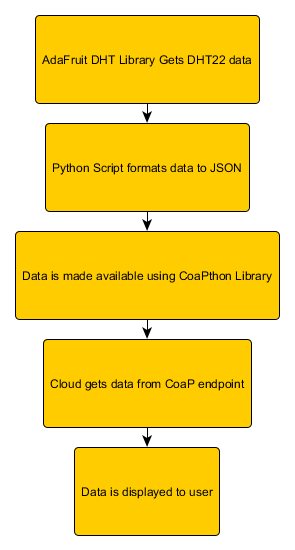
\includegraphics[width=0.5\textwidth]{assets/data_flow.png}}
    \caption{\label{fig:data_flow} Shows the flow of data from sensor to user.}
\end{figure}


\section{\gls{coap}-based \gls{iot} Architecture Components}
The aim of the proposed system is to investigate the implementation of \gls{coap} on a \gls{rpi} and how \gls{coap} can be 
used to transmit data to the cloud. 

To achieve this a \gls{coap} endpoint will need to be created on the \gls{rpi}. The \gls{rpi} will collect sensor data at intervals and store them 
locally on the device. The \gls{rpi} will act as a \gls{coap} server that will respond to \gls{rest} GET requests with the sensor data and the time
the reading was taken in a \gls{json} format.

The clouds responsibility will be to send the GET requests to the \gls{coap} endpoint hosted on the \gls{rpi} and to receive and store the data
returned. The cloud should send a confirmable request to the \gls{coap} endpoint. The \gls{coap} endpoint should then respond with an acknowledgement. 
If the data is available, the data should be ``piggybacked'' to this response, as shown in Figure \figref{fig:coap_get_piggy}, if not the data should be 
returned in a confirmable message containing the data.
 In this case the cloud client will then send it's own acknowledgement message to the \gls{coap} endpoint. This is shown in  \figref{fig:coap_get_delayed}.

\begin{figure}[H]
    \centering
    \makebox[1\textwidth]{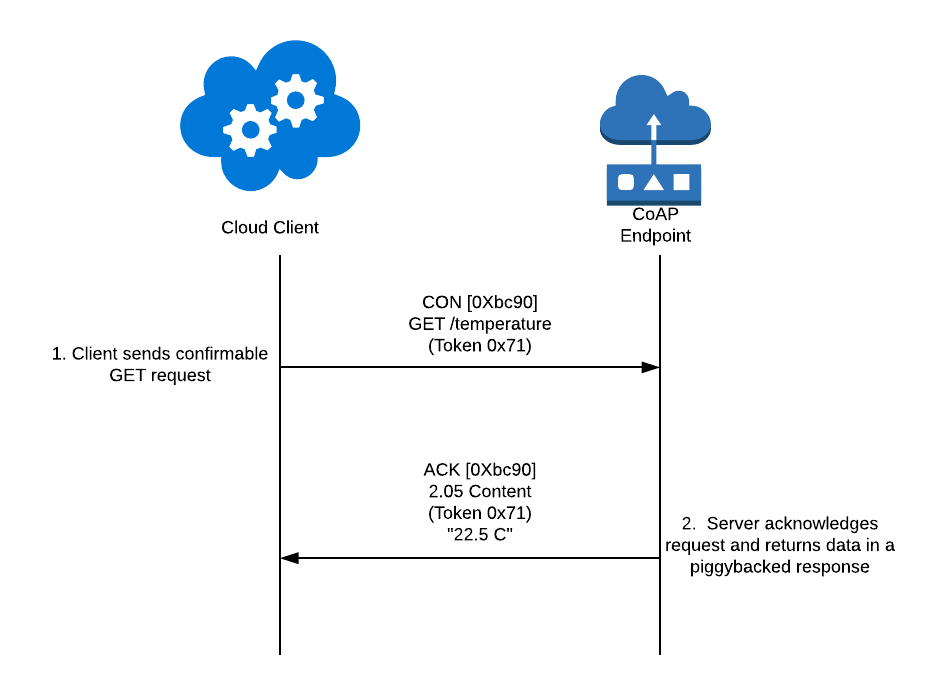
\includegraphics[width=1\textwidth]{assets/coap_get_request.png}}
    \caption{\label{fig:coap_get_piggy} Example \gls{coap} GET request with piggybacked response. \citep{bormann2015constrained}}
\end{figure}

With \gls{coap} endpoints acting as both a client, that sends requests, and a server implementation of \gls{coap} will be needed 
in each the \gls{rpi} and the cloud platform. The \gls{rpi} will then regularly retrieve readings from the sensor and send a POST request 
at intervals to the cloud \gls{coap} endpoint. This approach will be contrasted with the cloud server observing the \gls{rest} endpoint on the \gls{rpi}.
The results of both approaches will be evaluated.

\begin{figure}[H]
    \centering
    \makebox[1\textwidth]{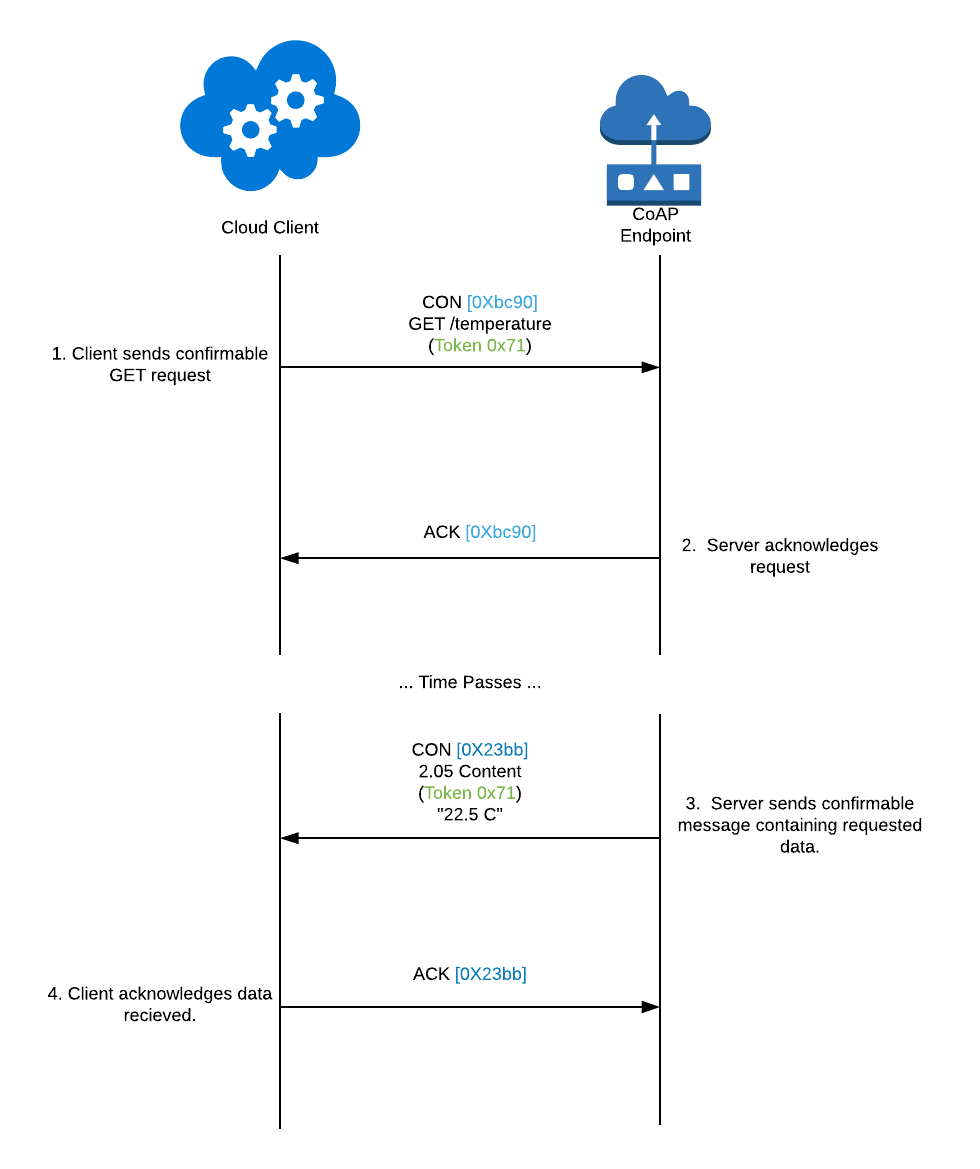
\includegraphics[width=1\textwidth]{assets/coap_get_delayed.png}}
    \caption{\label{fig:coap_get_delayed} Example \gls{coap} GET request without piggybacked response. \citep{bormann2015constrained}}
\end{figure}

\subsection{Hardware}
\begin{enumerate}
    \item Raspberry Pi 3

        Raspberry Pi 3 Model B, includes built in WiFi, \gls{gpio} ports and a 1.2GHz Quad-Core processor.
    \item Micro SD card
    
        Used to load operating system onto the \gls{rpi}.
    \item Power cord
    
        Supplies power to the \gls{rpi}.
    \item DHT22 temperature and humidity sensor
    
        Connects to the \gls{rpi} using the \gls{rpi}'s \gls{gpio} ports. Will be used to provide data.

\end{enumerate}

\subsection{Software}
\begin{enumerate}
    \item Python 3

        The Python programming language will be used to create the scripts and software needed on the \gls{rpi}.
        This is due to the languages popularity when creating projects on the \gls{rpi} and the languages wide selection
        of networking packages.
    \item CoAPthon
    
        Python implementation of \gls{coap}. Licensed under the MIT license. \href{https://github.com/Tanganelli/CoAPthon}{Github}.

    \item AdaFruit Python DHT
        
        Python library to retrieve sensor data from the DHT22. \href{https://github.com/adafruit/Adafruit_Python_DHT}{Github}.

    \item Git Version Control
    
        Source code version control system to allow for adjustments to the code.

    \item Cloud Platform
    
        Will act as an end point to the \gls{rpi} where the sensor data will be stored.
\end{enumerate}

\section{Conclusion and Future Work}
This research investigates the use of \gls{coap} in transmitting sensor data
to the cloud. It aims to explore how \gls{coap} fits into the \gls{iot} ecosystem and
what advantages, if any, it offers to other protocols. It also shows how a \gls{rpi} can
be used with Python to create an \gls{iot} device and connect to the cloud. 
Further work can be done with the data once it has been sent to the cloud.
The ThingsBoard platform offers many options with regards to actions performed,
based on data received from the \gls{iot} devices. Setting up alerts when data
falls outside of expected ranges, and sending messages to other \gls{iot} 
devices as a result, would allow this study to be applied to other uses such
as smart home automation. It would also be of interest to connect an 
actuator to the \gls{rpi} and see how this could be manipulated based on
\gls{coap} messages sent from the cloud. 

\printbibliography
\vspace{12pt}

\end{document}
